% Options for packages loaded elsewhere
\PassOptionsToPackage{unicode}{hyperref}
\PassOptionsToPackage{hyphens}{url}
\PassOptionsToPackage{dvipsnames,svgnames*,x11names*}{xcolor}
%
\documentclass[
  12pt,
  a4paper,
  12pt,
  oneside,
  openany]{book}
\usepackage{lmodern}
\usepackage{amssymb,amsmath}
\usepackage{ifxetex,ifluatex}
\ifnum 0\ifxetex 1\fi\ifluatex 1\fi=0 % if pdftex
  \usepackage[T1]{fontenc}
  \usepackage[utf8]{inputenc}
  \usepackage{textcomp} % provide euro and other symbols
\else % if luatex or xetex
  \usepackage{unicode-math}
  \defaultfontfeatures{Scale=MatchLowercase}
  \defaultfontfeatures[\rmfamily]{Ligatures=TeX,Scale=1}
  \setmainfont[]{DejaVu Serif}
  \setmonofont[Scale=0.8]{DejaVu Sans Mono}
\fi
% Use upquote if available, for straight quotes in verbatim environments
\IfFileExists{upquote.sty}{\usepackage{upquote}}{}
\IfFileExists{microtype.sty}{% use microtype if available
  \usepackage[]{microtype}
  \UseMicrotypeSet[protrusion]{basicmath} % disable protrusion for tt fonts
}{}
\makeatletter
\@ifundefined{KOMAClassName}{% if non-KOMA class
  \IfFileExists{parskip.sty}{%
    \usepackage{parskip}
  }{% else
    \setlength{\parindent}{0pt}
    \setlength{\parskip}{6pt plus 2pt minus 1pt}}
}{% if KOMA class
  \KOMAoptions{parskip=half}}
\makeatother
\usepackage{xcolor}
\IfFileExists{xurl.sty}{\usepackage{xurl}}{} % add URL line breaks if available
\IfFileExists{bookmark.sty}{\usepackage{bookmark}}{\usepackage{hyperref}}
\hypersetup{
  pdftitle={Devdoc-Swissknife EN},
  pdfauthor={Nikolay Gniteev},
  colorlinks=true,
  linkcolor=Maroon,
  filecolor=Maroon,
  citecolor=Blue,
  urlcolor=Blue,
  pdfcreator={LaTeX via pandoc}}
\urlstyle{same} % disable monospaced font for URLs
\usepackage{color}
\usepackage{fancyvrb}
\newcommand{\VerbBar}{|}
\newcommand{\VERB}{\Verb[commandchars=\\\{\}]}
\DefineVerbatimEnvironment{Highlighting}{Verbatim}{commandchars=\\\{\}}
% Add ',fontsize=\small' for more characters per line
\usepackage{framed}
\definecolor{shadecolor}{RGB}{248,248,248}
\newenvironment{Shaded}{\begin{snugshade}}{\end{snugshade}}
\newcommand{\AlertTok}[1]{\textcolor[rgb]{0.33,0.33,0.33}{#1}}
\newcommand{\AnnotationTok}[1]{\textcolor[rgb]{0.37,0.37,0.37}{\textbf{\textit{#1}}}}
\newcommand{\AttributeTok}[1]{\textcolor[rgb]{0.61,0.61,0.61}{#1}}
\newcommand{\BaseNTok}[1]{\textcolor[rgb]{0.06,0.06,0.06}{#1}}
\newcommand{\BuiltInTok}[1]{#1}
\newcommand{\CharTok}[1]{\textcolor[rgb]{0.5,0.5,0.5}{#1}}
\newcommand{\CommentTok}[1]{\textcolor[rgb]{0.37,0.37,0.37}{\textit{#1}}}
\newcommand{\CommentVarTok}[1]{\textcolor[rgb]{0.37,0.37,0.37}{\textbf{\textit{#1}}}}
\newcommand{\ConstantTok}[1]{\textcolor[rgb]{0,0,0}{#1}}
\newcommand{\ControlFlowTok}[1]{\textcolor[rgb]{0.27,0.27,0.27}{\textbf{#1}}}
\newcommand{\DataTypeTok}[1]{\textcolor[rgb]{0.27,0.27,0.27}{#1}}
\newcommand{\DecValTok}[1]{\textcolor[rgb]{0.06,0.06,0.06}{#1}}
\newcommand{\DocumentationTok}[1]{\textcolor[rgb]{0.37,0.37,0.37}{\textbf{\textit{#1}}}}
\newcommand{\ErrorTok}[1]{\textcolor[rgb]{0.14,0.14,0.14}{\textbf{#1}}}
\newcommand{\ExtensionTok}[1]{#1}
\newcommand{\FloatTok}[1]{\textcolor[rgb]{0.06,0.06,0.06}{#1}}
\newcommand{\FunctionTok}[1]{\textcolor[rgb]{0,0,0}{#1}}
\newcommand{\ImportTok}[1]{#1}
\newcommand{\InformationTok}[1]{\textcolor[rgb]{0.37,0.37,0.37}{\textbf{\textit{#1}}}}
\newcommand{\KeywordTok}[1]{\textcolor[rgb]{0.27,0.27,0.27}{\textbf{#1}}}
\newcommand{\NormalTok}[1]{#1}
\newcommand{\OperatorTok}[1]{\textcolor[rgb]{0.43,0.43,0.43}{\textbf{#1}}}
\newcommand{\OtherTok}[1]{\textcolor[rgb]{0.37,0.37,0.37}{#1}}
\newcommand{\PreprocessorTok}[1]{\textcolor[rgb]{0.37,0.37,0.37}{\textit{#1}}}
\newcommand{\RegionMarkerTok}[1]{#1}
\newcommand{\SpecialCharTok}[1]{\textcolor[rgb]{0,0,0}{#1}}
\newcommand{\SpecialStringTok}[1]{\textcolor[rgb]{0.5,0.5,0.5}{#1}}
\newcommand{\StringTok}[1]{\textcolor[rgb]{0.5,0.5,0.5}{#1}}
\newcommand{\VariableTok}[1]{\textcolor[rgb]{0,0,0}{#1}}
\newcommand{\VerbatimStringTok}[1]{\textcolor[rgb]{0.5,0.5,0.5}{#1}}
\newcommand{\WarningTok}[1]{\textcolor[rgb]{0.37,0.37,0.37}{\textbf{\textit{#1}}}}
\usepackage{longtable,booktabs}
% Correct order of tables after \paragraph or \subparagraph
\usepackage{etoolbox}
\makeatletter
\patchcmd\longtable{\par}{\if@noskipsec\mbox{}\fi\par}{}{}
\makeatother
% Allow footnotes in longtable head/foot
\IfFileExists{footnotehyper.sty}{\usepackage{footnotehyper}}{\usepackage{footnote}}
\makesavenoteenv{longtable}
\usepackage{graphicx}
\makeatletter
\def\maxwidth{\ifdim\Gin@nat@width>\linewidth\linewidth\else\Gin@nat@width\fi}
\def\maxheight{\ifdim\Gin@nat@height>\textheight\textheight\else\Gin@nat@height\fi}
\makeatother
% Scale images if necessary, so that they will not overflow the page
% margins by default, and it is still possible to overwrite the defaults
% using explicit options in \includegraphics[width, height, ...]{}
\setkeys{Gin}{width=\maxwidth,height=\maxheight,keepaspectratio}
% Set default figure placement to htbp
\makeatletter
\def\fps@figure{htbp}
\makeatother
\setlength{\emergencystretch}{3em} % prevent overfull lines
\providecommand{\tightlist}{%
  \setlength{\itemsep}{0pt}\setlength{\parskip}{0pt}}
\setcounter{secnumdepth}{5}
\usepackage[]{natbib}
\bibliographystyle{apalike}

\title{Devdoc-Swissknife EN}
\author{Nikolay Gniteev}
\date{2022-05-14}

\begin{document}
\maketitle

{
\hypersetup{linkcolor=}
\setcounter{tocdepth}{2}
\tableofcontents
}
\listoftables
\listoffigures
\hypertarget{intro}{%
\chapter*{Preface}\label{intro}}


This is a demo project for development documentation generation with \href{https://rmarkdown.rstudio.com/}{\textbf{R Markdown}} and \href{https://kroki.io/}{\textbf{Kroki}}.

All the things described here you could do without that project, but I've tried to stich those components together so you'll be able to concentrate on content rather than process.

This approach allows you to create reproducible documentation in form of PDF, presentations, gitbook and some other HTML formats from simple markdown-like files (Pandoc flavor) with extra \textbf{R chunks} and textual diagrams description.

The goal of this project is to describe documentation via text files as much as possible, even graphic diagrams, and make it easy to use without overcomplication.

A textual description provides an easy way to version and merge diagrams, get differences between versions, leave comments that stays out from generated documentation, review changes, etc.

Also most often it's faster to create and \textbf{edit} diagrams as text, do things like theming and refactoring themes. Since the diagram's textual description often is more a model than just graphics, you don't have to track existing objects relations when just placement is changed or objects added (until you rename objects) which makes your workflow less error-prone.

Embedding textually described diagrams into docuement is the actual focus of this porject. The rest you would be able to do with R Markdown itself as it is a powerful and customizable tool, so you can fit docs to your needs. It would take efforts on start, to make things neat but it would repay you in the end.

\begin{quote}
To produce awesome PDFs you'll have to provide awesome Latex book class. Since I don't have one I'm using Latex default so current PDF version looks a bit ugly to me. I hope I can fix this soon or later. Help is appreciated!
\end{quote}

Kroki is running locally in container so you may not worry for confidential things and it works well in air gapped installations.

\begin{center}\rule{0.5\linewidth}{0.5pt}\end{center}

This project is also can be used as a template for your own documentation, see \protect\hyperlink{template}{this section}

The project uses docker and docker-compose to build docs so it's ready to be integrated into your CI/CD flow.

The project's structure, docs generation and some files are based on \href{https://github.com/rstudio/rmarkdown-book}{R Markdown book}

\begin{center}\rule{0.5\linewidth}{0.5pt}\end{center}

There are few demonstrations in the project for general development use-cases (which probably cover 95\% of your daily needs). For more complicated use-cases - checkout docs on links below.

\begin{quote}
Diagrams code for most examples is borrowed straight from \href{https://kroki.io/examples.html}{Kroki}
\end{quote}

\begin{center}\rule{0.5\linewidth}{0.5pt}\end{center}

\protect\hyperlink{usage}{Usage} section would be updated eventually with reciepes for common cases.

\hfill\break
\hfill\break

\hypertarget{links}{%
\subsection*{Helpful links}\label{links}}


\hypertarget{links-diagrams}{%
\subsubsection*{Diagrams}\label{links-diagrams}}


\href{https://kroki.io/\#support}{List of supported diagrams renderers}

\href{https://kroki.io/examples.html}{A few more diagrams examples}

\hypertarget{links-rmarkdown}{%
\subsubsection*{R Markdown}\label{links-rmarkdown}}


\href{https://bookdown.org/yihui/rmarkdown/}{R Markdown: The Definitive Guide}

\href{https://bookdown.org/yihui/rmarkdown-cookbook/}{R Markdown: Cookbook}

\href{https://bookdown.org/yihui/bookdown/}{Bookdown: Authoring Books and Technical Docuements with R Markdown}

\href{https://rmarkdown.rstudio.com/lesson-1.html}{R Markdown Site} (focused on usage with \textbf{R Studio})

\href{https://rmd4sci.njtierney.com/}{A nice R Markdown tutorial}

\href{https://rmarkdown.rstudio.com/docs/reference/index.html}{R Markdown reference}

\hypertarget{links-rmarkdown-quick}{%
\subsubsection*{Get quick into R Markdown}\label{links-rmarkdown-quick}}


\href{https://intro2r.com/r-markdown-anatomy.html}{R Makedown anatomy}

\href{https://www.rstudio.com/wp-content/uploads/2015/03/rmarkdown-reference.pdf}{R Markdown short reference} to get familiar with most necessary things

\href{https://raw.githubusercontent.com/rstudio/cheatsheets/master/rmarkdown.pdf}{R Markdown cheatsheet}

\hypertarget{links-editors}{%
\subsubsection*{Editors with focus on diagrams}\label{links-editors}}


\href{https://github.com/DaveJarvis/keenwrite}{\textbf{Keenwrite} - edit and preview R Markdown Live!}

\href{https://www.rstudio.com/}{\textbf{R Studio}}

\hypertarget{links-alternatives}{%
\subsection*{Alternatives}\label{links-alternatives}}


\url{https://bookdown.org/yihui/rmarkdown-cookbook/diagrams.html} / \url{https://rich-iannone.github.io/DiagrammeR/}

\hypertarget{examples}{%
\chapter{Simple diagrams examples}\label{examples}}

Since this project is focused on embedding diagrams textual descriptions into \textbf{R Markdown}, let's start with few examples just to illustrate a principle.

\begin{quote}
BTW: there is a lot of drawings types that you can get from \textbf{R Markdown} alone, by using \textbf{R} packages or Python's matplot lib for example. You may want to check this out too.
\end{quote}

\hypertarget{examples-inline}{%
\subsection*{Example with inline diagram description}\label{examples-inline}}


This example shows how to embed diagrams, describing them right in the \texttt{.Rmd} files.

\begin{Shaded}
\begin{Highlighting}[]
\StringTok{\textasciigrave{}\textasciigrave{}\textasciigrave{}}\DataTypeTok{\{r, hello{-}world, dia="graphviz", fig.cap="Hello World"\}}
\DataTypeTok{  to\_diagram("digraph G \{Hello{-}\textgreater{}World\}")}
\StringTok{\textasciigrave{}\textasciigrave{}\textasciigrave{}}
\end{Highlighting}
\end{Shaded}

\begin{figure}

{\centering 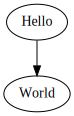
\includegraphics[height=4cm]{generated/hello-world} 

}

\caption{Hello World}\label{fig:hello-world}
\end{figure}

\newpage

\hypertarget{examples-fromFile}{%
\subsection*{Example with diagram data from file}\label{examples-fromFile}}


This example shows how to embed diagrams with data from outer files.

\small

\begin{Shaded}
\begin{Highlighting}[]
\StringTok{\textasciigrave{}\textasciigrave{}\textasciigrave{}}\DataTypeTok{\{r, examples{-}entity{-}relation, dia="erd", fig.cap="Entity Relation"\}}
\DataTypeTok{  to\_diagram(src="../diagrams/examples/project.erd")}
\StringTok{\textasciigrave{}\textasciigrave{}\textasciigrave{}}
\end{Highlighting}
\end{Shaded}

\normalsize

\begin{figure}

{\centering 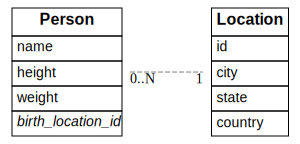
\includegraphics[width=8cm]{generated/diagrams-examples-project-erd} 

}

\caption{Entity Relation}\label{fig:examples-entity-relation}
\end{figure}

\newpage

File \textbf{diagrams/examples/project.erd} content:

\begin{verbatim}
[Person]
*name
height
weight
+birth_location_id

[Location]
*id
city
state
country

Person *--1 Location
\end{verbatim}

\hypertarget{examples-more}{%
\subsection*{More examples}\label{examples-more}}


More examples for your inspiration can be found in \protect\hyperlink{examples-kroki}{this section}.

Details about embedding diagrams is \protect\hyperlink{usage}{here}

\hypertarget{template}{%
\chapter{Using as a template and making own docs}\label{template}}

To use this project as a start point for generating your own documentation do the following:

\begin{enumerate}
\def\labelenumi{\arabic{enumi}.}
\tightlist
\item
  Import project and prepare for making docs
\end{enumerate}

\begin{quote}
You'll need to have already \texttt{docker} and \texttt{docker-compose} installed
\end{quote}

\begin{itemize}
\item
  Import or fork main branch of this repo: \url{https://github.com/Godhart/devdoc-swissknife}.\\
  All the sources for docs are contained in \texttt{docs\_src} folder.
\item
  Make docker image \texttt{devdoc-swissknife} if you don't have one already.\\
  Simply run \texttt{make\_docker.sh} from \texttt{docker} dir.
\item
  Ensure that everything works fine - try to make docs with \texttt{make\_docs.sh}.\\
  Output docs should appear in \texttt{docs\_out/devdoc-swissknife-*} folders. Check that docs exist and contain graphics.\\
  \emph{Take a NOTE: \texttt{docs\_out} folder and all it's content is ignored by git.}
\item
  If you don't want to see devdoc-swissknife documentation in your repo:

  \begin{itemize}
  \tightlist
  \item
    Remove \texttt{docs\_src/devdoc-swissknife-*} folders
  \item
    Remove \texttt{docs\_out/devdoc-swissknife-*} folders
  \item
    Empty \texttt{docs\_src/diagrams} folder.
  \end{itemize}
\end{itemize}

\begin{enumerate}
\def\labelenumi{\arabic{enumi}.}
\setcounter{enumi}{1}
\tightlist
\item
  Prepare for making your own docs
\end{enumerate}

\begin{itemize}
\item
  Make a new folder in \texttt{docs\_src}. I suggest you name it using the following pattern: \texttt{doc-\textless{}subject\textgreater{}}
\item
  Copy all the files from \texttt{docs\_src/docs-template} into your brand new folder
\item
  Replace following keywords \texttt{\textless{}Author\ Name\textgreater{}}, \texttt{\textless{}author\textgreater{}}, \texttt{\textless{}repo\textgreater{}}, \texttt{\textless{}Document\ Title\textgreater{}}, \texttt{Document\_Title}, \texttt{\textless{}Document\ Description\textgreater{}}, doc- within files in your new folder with actual values. Also don't forget to adjust \texttt{Document\_Title} in the \texttt{.gitignore} of new folder, as it protects from build garbage.
\item
  Adjust \texttt{docs\_src/Makefile} to fit your needs (for the first time - use an existing pattern to add your folder).
\item
  Ensure that everything is still fine - try to make docs with \texttt{make\_docs.sh}.\\
  Output docs should appear in \texttt{docs\_out/doc-\textless{}subject\textgreater{}} folder if you followed a pattern in the Makefile.
\end{itemize}

\begin{quote}
NOTE: in many cases of errors doc's sources folder (\texttt{docs\_src/doc-\textless{}subject\textgreater{}} if you follow suggested pattern) is polluted with temporary files, named as specified in \texttt{\_bookdown.yml} (field \texttt{book\_filename}) and may break following docs generation runs.\\
These files are removed with make routine, but in some cases, you'll have to remove them by yourself.\\
Changing \texttt{book\_filename} field in \texttt{\_bookdown.yml} after an error has happened may be the case.
\end{quote}

\begin{enumerate}
\def\labelenumi{\arabic{enumi}.}
\setcounter{enumi}{2}
\tightlist
\item
  Create content
\end{enumerate}

\begin{itemize}
\item
  Update \texttt{index.Rmd} in your folder to your needs (contains \emph{Preface} section).
\item
  Add your own docs into your folder, naming files like \texttt{\textless{}number\textgreater{}-\textless{}chapter-name\textgreater{}.Rmd}.\\
  Check the \textbf{R Markdown} and \textbf{Kroki} docs for understanding things. Also, you may rely on shown examples.
\item
  If you already have docs in markdown format you may already use them like this:

  \begin{itemize}
  \tightlist
  \item
    copy markdown files into your doc-folder
  \item
    copy necessary local images to location in \texttt{docs\_src/diagrams} or wherever you like most
  \item
    change name extensions of markdown files to \texttt{.Rmd}
  \item
    change names of markdown files so they would correspond to pattern \texttt{\textless{}number\textgreater{}-\textless{}chapter-name\textgreater{}.Rmd}
  \item
    change references to local images in markdown files
  \end{itemize}
\item
  If you already have text description of diagrams for supported rendering engines you may already use them like this:

  \begin{itemize}
  \tightlist
  \item
    copy necessary files to location in \texttt{docs\_src/diagrams} or wherever you like most
  \item
    in \texttt{.Rmd} files replace image embedding with diagram embedding as described \url{TODO}
  \end{itemize}
\item
  Most probably you would like to use your own Latex class, so add \texttt{\textless{}your\_latex\_class\textgreater{}.cls} file into your folder and specify it in \texttt{index.Rmd} file (replace \texttt{documentclass:\ book} field with \texttt{\textless{}your\_latex\_class\textgreater{}} name).
\end{itemize}

\begin{quote}
Adding custom latex class may require you to add some latex packages to Docker image. Same is true if you do use some special \textbf{R} packages in your docs etc.\\
If this is the case you'll have to modify \texttt{docker/Dockerfile} and build again docker image with \texttt{make\_docker.sh}.
\end{quote}

\hypertarget{examples-kroki}{%
\chapter{Kroki usage examples}\label{examples-kroki}}

I've omitted some examples from \href{https://kroki.io/examples.html}{Kroki} and left only those that are most useful in a daily life of most developers (IMO).

If you check docs for \href{https://kroki.io/\#support}{supported diagrams renderers} then you'll find for sure a few more interesting usecases.

All diagrams data for examples of this section resides in \href{https://github.com/Godhart/devdoc-swissknife/tree/main/docs_src/diagrams/examples}{docs\_src/diagrams/examples} dir of this repo. Each diagram is included into doc by adding following code section into document file:

\begin{Shaded}
\begin{Highlighting}[]
\StringTok{\textasciigrave{}\textasciigrave{}\textasciigrave{}}\DataTypeTok{\{r, \textless{}reference{-}label\textgreater{}, dia="from\_src", fig.cap="\textless{}Caption for your figure\textgreater{}"\}}
\DataTypeTok{  to\_diagram(src="../diagrams/\textless{}src\_file\_path\_within\_diagrams\_dir\textgreater{}")}
\StringTok{\textasciigrave{}\textasciigrave{}\textasciigrave{}}
\end{Highlighting}
\end{Shaded}

Full code for this whole section is \href{https://github.com/Godhart/devdoc-swissknife/blob/main/docs_src/devdoc-swissknife-en/03-KrokiExamples.Rmd}{here}

This usage pattern is described in the following section \protect\hyperlink{TODO}{TODO}

\newpage

\hypertarget{kroki-c4context}{%
\section{C4 Context Diagram (PlantUML+C4)}\label{kroki-c4context}}

Engine: \texttt{c4plantuml}

\begin{figure}

{\centering 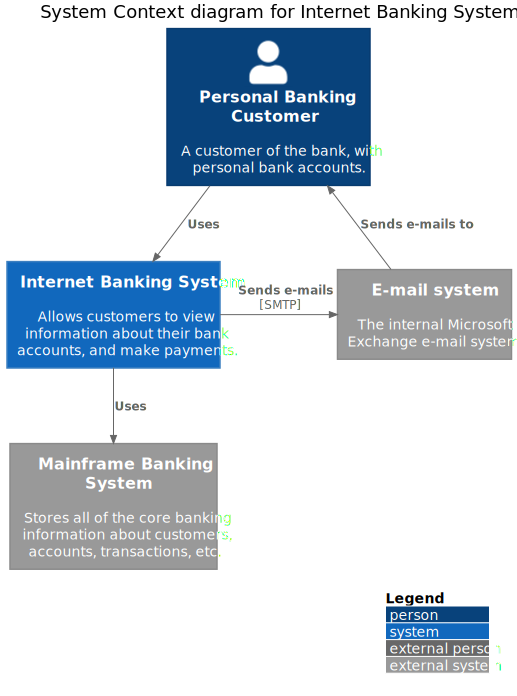
\includegraphics[height=15cm]{generated/diagrams-examples-c4plantuml-context-Rmd} 

}

\caption{Example - C4 Context Diagram}\label{fig:examples-c4context}
\end{figure}

\begin{quote}
*NOTE: inserted as PNG image due to errors in SVG to PDF conversion
\end{quote}

\newpage

\hypertarget{kroki-c4container}{%
\section{C4 Container Diagram (PlantUML+C4)}\label{kroki-c4container}}

Engine: \texttt{c4plantuml}

\begin{figure}

{\centering 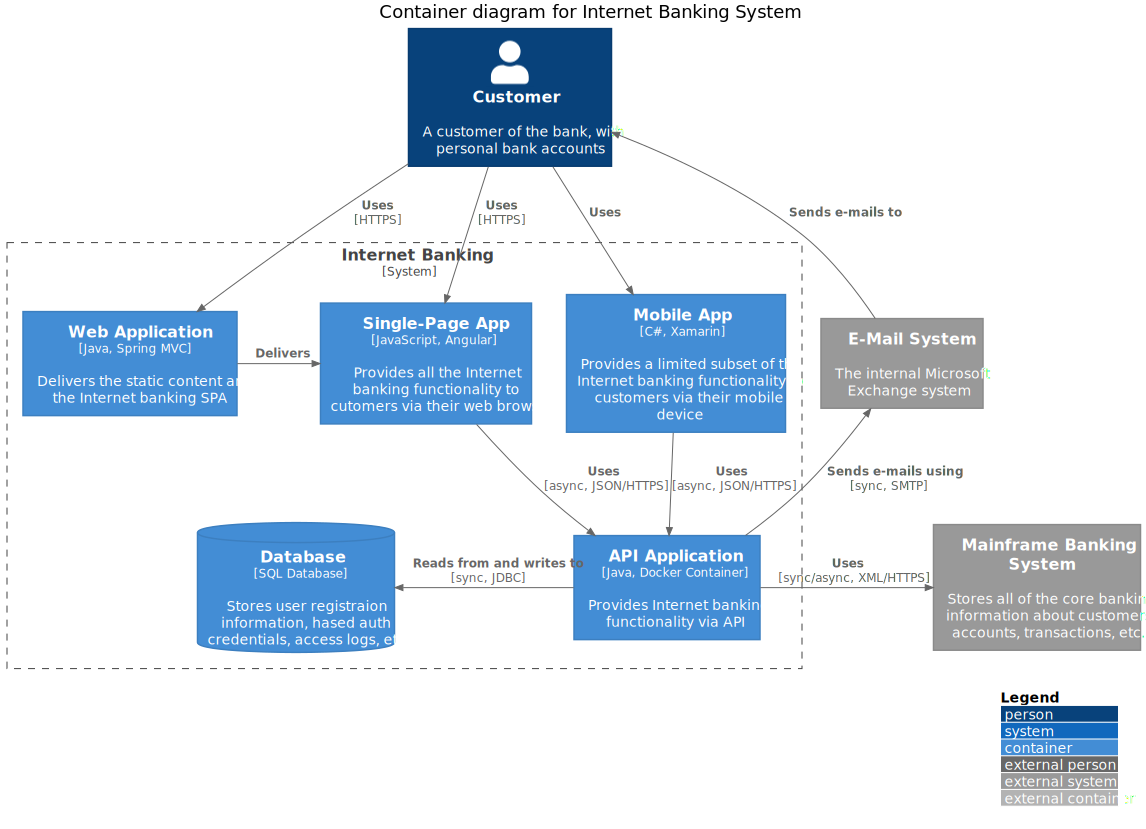
\includegraphics{generated/diagrams-examples-c4plantuml-container-Rmd} 

}

\caption{Example - C4 Container Diagram}\label{fig:examples-c4container}
\end{figure}

\begin{quote}
*NOTE: inserted as PNG image due to errors in SVG to PDF conversion
\end{quote}

\newpage

\hypertarget{kroki-c4component}{%
\section{C4 Component Diagram (PlantUML+C4)}\label{kroki-c4component}}

Engine: \texttt{c4plantuml}

\begin{figure}

{\centering 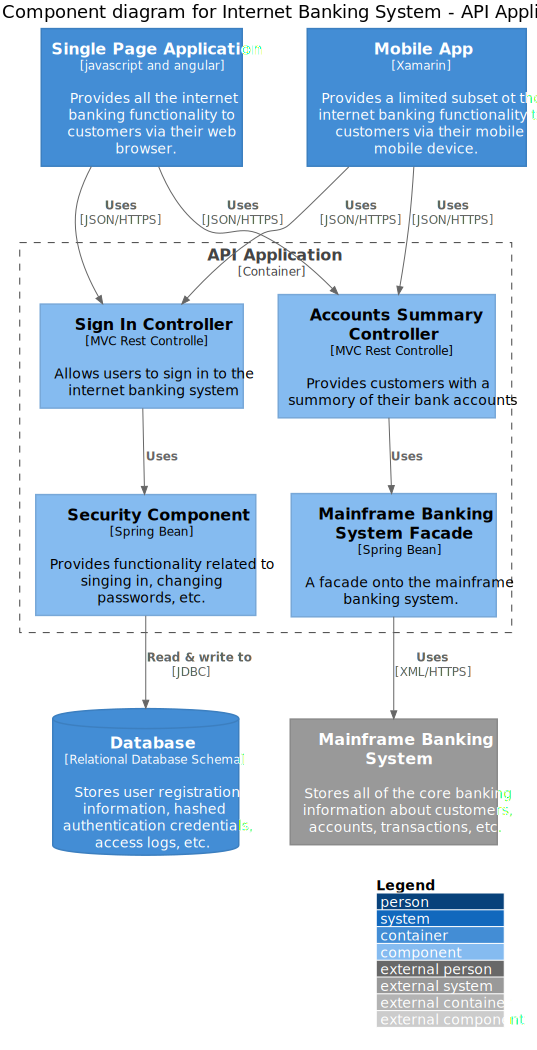
\includegraphics[height=15cm]{generated/diagrams-examples-c4plantuml-component-Rmd} 

}

\caption{Example - C4 Component Diagram}\label{fig:examples-c4component}
\end{figure}

\begin{quote}
*NOTE: inserted as PNG image due to errors in SVG to PDF conversion
\end{quote}

\newpage

\hypertarget{kroki-blockdiag}{%
\section{Block Diagram}\label{kroki-blockdiag}}

Engine: \texttt{blockdiag}

\begin{figure}

{\centering 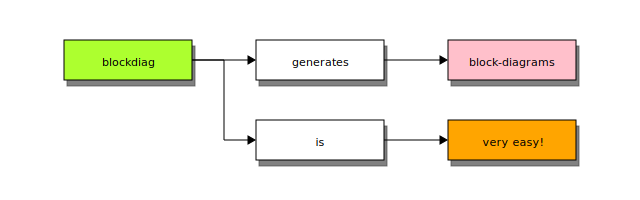
\includegraphics{generated/diagrams-examples-blockdiag-Rmd} 

}

\caption{Example - Block Diagram}\label{fig:examples-blockdiag}
\end{figure}

\newpage

\hypertarget{kroki-timing}{%
\section{Digital Timing Diagram}\label{kroki-timing}}

Engine: \texttt{wavedrom}

\begin{figure}

{\centering 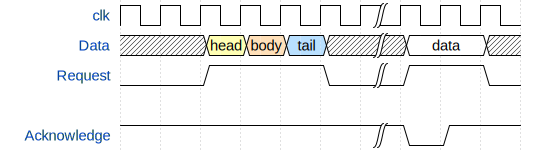
\includegraphics{generated/diagrams-examples-wavedrom-Rmd} 

}

\caption{Example - Digital Timing Diagram}\label{fig:examples-timing}
\end{figure}

\newpage

\hypertarget{kroki-bytefield}{%
\section{Bytefield}\label{kroki-bytefield}}

Engine: \texttt{bytefield}

\begin{figure}

{\centering 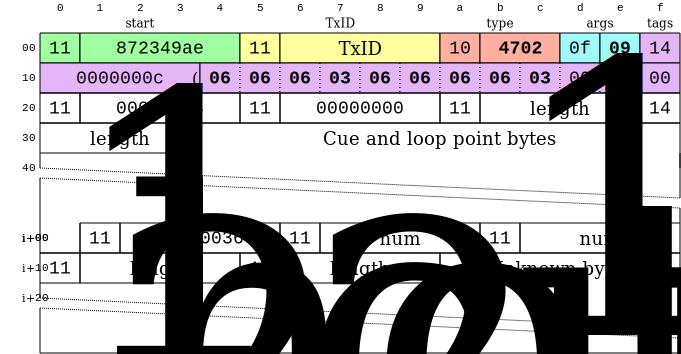
\includegraphics{generated/diagrams-examples-bytefield-Rmd} 

}

\caption{Example - Bytefield}\label{fig:examples-bytefield}
\end{figure}

\newpage

\hypertarget{kroki-packet}{%
\section{Packet Diagram}\label{kroki-packet}}

Engine: \texttt{packetdiag}

\begin{figure}

{\centering 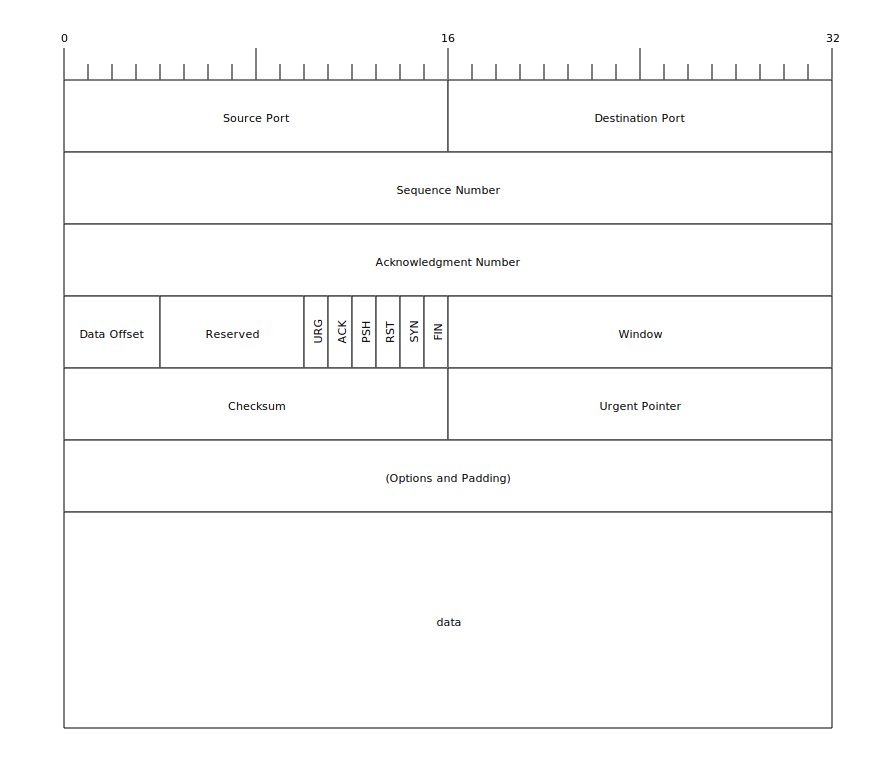
\includegraphics{generated/diagrams-examples-packetdiag-Rmd} 

}

\caption{Example - Packet Diagram}\label{fig:examples-packet}
\end{figure}

\newpage

\hypertarget{kroki-pumlSequence}{%
\section{Sequence Diagram \#1 (PlantUML)}\label{kroki-pumlSequence}}

Engine: \texttt{plantuml}

\begin{figure}

{\centering 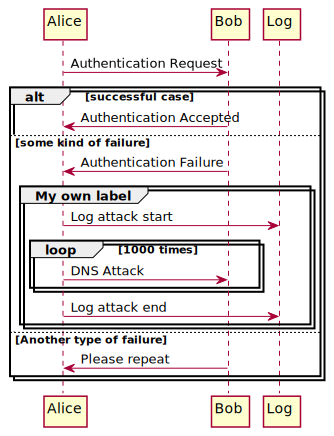
\includegraphics[height=15cm]{generated/diagrams-examples-plantuml-seqdiag-Rmd} 

}

\caption{Example - Sequence Diagram - PlantUML}\label{fig:examples-pumlSequence}
\end{figure}

\newpage

\hypertarget{kroki-sequence}{%
\section{Sequence Diagram \#2 (SeqDiag)}\label{kroki-sequence}}

Engine: \texttt{seqdiag}

\begin{figure}

{\centering 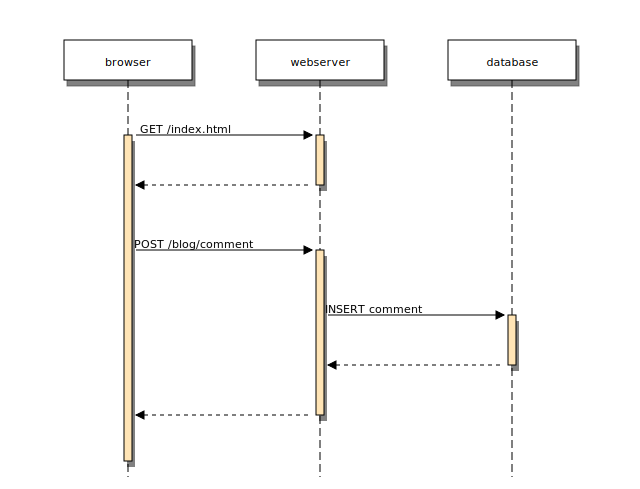
\includegraphics{generated/diagrams-examples-seqdiag-Rmd} 

}

\caption{Example - Sequence Diagram - SeqDiag}\label{fig:examples-sequence}
\end{figure}

\newpage

\hypertarget{kroki-commitgraph}{%
\section{Commit Graph}\label{kroki-commitgraph}}

Engine: \texttt{pikchr}

\begin{quote}
\emph{NOTE: pikchr is giving troubles in PDF/PNG (produced SVG output is only web-browser friendly)}\\
\emph{That's why this diagram is absent in PDF version}
\end{quote}

\newpage

\hypertarget{kroki-pumlUsecase}{%
\section{Use Case Diagram}\label{kroki-pumlUsecase}}

Engine: \texttt{plantuml}

\begin{figure}

{\centering 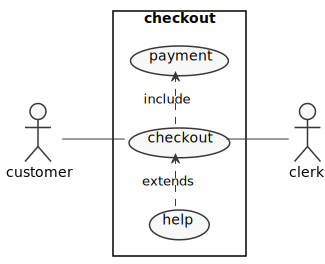
\includegraphics{generated/diagrams-examples-plantuml-usecase-Rmd} 

}

\caption{Example Block Diagram}\label{fig:examples-pumlUsecase}
\end{figure}

\newpage

\hypertarget{kroki-pumlMindmap}{%
\section{Mind Map}\label{kroki-pumlMindmap}}

Engine: \texttt{plantuml}

\begin{figure}

{\centering 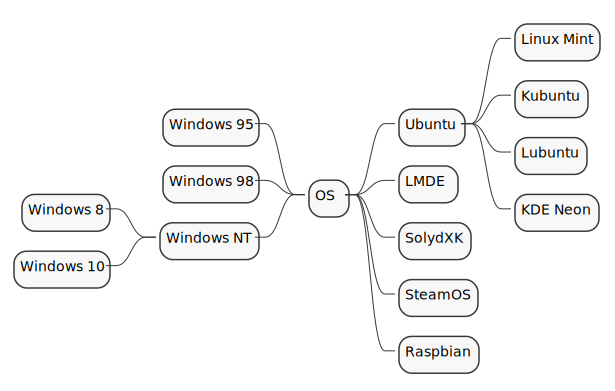
\includegraphics{generated/diagrams-examples-plantuml-mindmap-Rmd} 

}

\caption{Example - Mind Map}\label{fig:examples-pumlMindmap}
\end{figure}

\newpage

\hypertarget{kroki-pumlMore}{%
\section{PlantUML (More examples)}\label{kroki-pumlMore}}

PlantUML supports more diagram types like timing diagram, gantt and many more.

You can use any of them just like in previous examples.

Check PlantUML docs \url{https://plantuml.com/} for filling in diagram data.

\newpage

\hypertarget{kroki-gantt}{%
\section{Gantt}\label{kroki-gantt}}

Engine: \texttt{mermaid}

\begin{quote}
\emph{NOTE: mermaid is giving troubles in PDF/PNG (produced SVG output is only web-browser friendly)} \emph{That's why this diagram is absent in PDF version}
\end{quote}

\hypertarget{usage}{%
\chapter{Usage patterns}\label{usage}}

There are few proposed ways to embed diagrams into a document and to customize them.

Which one to use depends on circumstances.

\begin{quote}
This section would be updated as project evolves
\end{quote}

\hypertarget{usage-embed}{%
\section{Embedding diagrams into a document}\label{usage-embed}}

Let's cover basics on embedding diagrams into documentation first.

\hypertarget{usage-embed-inline}{%
\subsection{Describing diagrams inline in the documentation}\label{usage-embed-inline}}

Useful for short and/or strongly context-related drawings, i.e.~when drawing by itself have no meaning or there is no reason for storing it in a separate file.

Following pattern should be used:

\begin{Shaded}
\begin{Highlighting}[]
\StringTok{\textasciigrave{}\textasciigrave{}\textasciigrave{}}\DataTypeTok{\{r \textless{}label\textgreater{}, dia=\textquotesingle{}\textless{}engine\textgreater{}\textquotesingle{}, fig.cap=\textquotesingle{}\textless{}drawing name\textgreater{}\textquotesingle{}\}}
\DataTypeTok{  to\_diagram(\textquotesingle{}\textless{}diagram data\textgreater{}\textquotesingle{})}
\StringTok{\textasciigrave{}\textasciigrave{}\textasciigrave{}}
\end{Highlighting}
\end{Shaded}

where:

\begin{itemize}
\tightlist
\item
  \texttt{\textless{}label\textgreater{}} is a name for a drawing reference, may be omitted
\item
  \texttt{\textless{}engine\textgreater{}} is a name for a rendering engine, see \protect\hyperlink{reference-engines}{table} for allowed values and corresponding engines
\item
  \texttt{\textless{}drawing\ name\textgreater{}} is a caption for drawing, may be omitted.
\item
  \texttt{\textless{}diagram\ data\textgreater{}} is a textual diagram description in a format that is compatible with a rendering engine\\
  \emph{NOTE: if there are single quotes in the \texttt{\textless{}diagram\ data\textgreater{}} then you should escape them with \texttt{\textbackslash{}} symbol} \emph{or surround \texttt{\textless{}diagram\ data\textgreater{}} with double-quotes (\texttt{"}) instead.}
\end{itemize}

\hypertarget{usage-embed-raw}{%
\subsection{Diagrams from raw outer files}\label{usage-embed-raw}}

This is the case if you already have a diagram description in a separate file and you want to keep it like that for some reason.

\begin{quote}
For new diagrams it's proposed to use method, described in the next section. It also uses outer files, but requires some extra formating.
\end{quote}

Raw file is a text file that contains diagram description data in a format that is compatible with a rendering engine and nothing more.

Following pattern should be used:

\begin{Shaded}
\begin{Highlighting}[]
\StringTok{\textasciigrave{}\textasciigrave{}\textasciigrave{}}\DataTypeTok{\{r \textless{}label\textgreater{}, dia=\textquotesingle{}\textless{}engine\textgreater{}\textquotesingle{}, fig.cap=\textquotesingle{}\textless{}drawing name\textgreater{}\textquotesingle{}\}}
\DataTypeTok{  to\_diagram(src=\textquotesingle{}\textless{}src\_file\_path\textgreater{}\textquotesingle{})}
\StringTok{\textasciigrave{}\textasciigrave{}\textasciigrave{}}
\end{Highlighting}
\end{Shaded}

where:

\begin{itemize}
\tightlist
\item
  \texttt{\textless{}label\textgreater{}} is a name for a drawing reference, may be omitted
\item
  \texttt{\textless{}engine\textgreater{}} is a name for a rendering engine, see \protect\hyperlink{reference-engines}{table} for allowed values and corresponding engines
\item
  \texttt{\textless{}drawing\ name\textgreater{}} is a caption for drawing, mey be omitted
\item
  \texttt{\textless{}src\_file\_path\textgreater{}} is a path to file with diagram data, relative to file into which it's embedded.\\
  \emph{If you are using suggested locations to place docs and diagrams (\texttt{docs\_src/doc-\textless{}subject\textgreater{}} and \texttt{docs\_src/diagrams})} \emph{then value for \texttt{\textless{}src\_file\_path\textgreater{}} should be starting like this: \texttt{../diagrams/}}
\end{itemize}

\hypertarget{usage-embed-rmd}{%
\subsection{Diagrams from Rmd outer file}\label{usage-embed-rmd}}

This is a proposed way to describe diagrams in outer files. Diagram data should be in \texttt{.Rmd} file and described as specified in \texttt{docs\_src/diagrams/README.md} \url{TODO}.

This way you'll be able to use \href{https://github.com/DaveJarvis/keenwrite}{Keenwrite} to preview diagrams live while editing, which is very handy.

Besides that, you can supply a diagram with additional info, capture decisions that were taken, add TODOs, versions info, etc. along with diagram's data in the same file.

Following pattern should be used:

\begin{Shaded}
\begin{Highlighting}[]
\StringTok{\textasciigrave{}\textasciigrave{}\textasciigrave{}}\DataTypeTok{\{r \textless{}label\textgreater{}, dia=\textquotesingle{}from\_src\textquotesingle{}, fig.cap=\textquotesingle{}\textless{}drawing name\textgreater{}\textquotesingle{}\}}
\DataTypeTok{  to\_diagram(src=\textquotesingle{}\textless{}src\_file\_path\textgreater{}\textquotesingle{})}
\StringTok{\textasciigrave{}\textasciigrave{}\textasciigrave{}}
\end{Highlighting}
\end{Shaded}

where:

\begin{itemize}
\tightlist
\item
  \texttt{\textless{}label\textgreater{}} is a name for a drawing reference, may be omitted
\item
  \texttt{\textless{}drawing\ name\textgreater{}} is a caption for drawing, mey be omitted
\item
  \texttt{\textless{}src\_file\_path\textgreater{}} is a path to file with diagram data, relative file into which it's embedded.\\
  \emph{If you are using suggested locations to place docs and diagrams (\texttt{docs\_src/doc-\textless{}subject\textgreater{}} and \texttt{docs\_src/diagrams})} \emph{then value for \texttt{\textless{}src\_file\_path\textgreater{}} should be starting like this: \texttt{../diagrams/}}
\end{itemize}

\begin{quote}
Take a NOTE: A \texttt{from\_src} is specified as engine in this case since an actual engine name is already specified in \texttt{.Rmd} file with diagram data.
\end{quote}

\hypertarget{usage-embed-getThenEmbed}{%
\subsection{Get then embed}\label{usage-embed-getThenEmbed}}

This is the case if you want to customize diagrams embedding, like aligning, multiple diagrams in a single row, preprocess diagrams before embedding them, etc.

The process is divided into few phases:

\begin{enumerate}
\tightlist
\item
  Download one or multiple rendered images for your diagrams
\item
  Preprocess diagrams if required
\item
  Embed them into document
\end{enumerate}

\begin{quote}
NOTE: diagrams are still described in a text form
\end{quote}

Following pattern should be used:

\begin{Shaded}
\begin{Highlighting}[]
\CommentTok{\# Download diagram}
\StringTok{\textasciigrave{}\textasciigrave{}\textasciigrave{}}\DataTypeTok{\{r dia=\textquotesingle{}from\_src\textquotesingle{}\}}
\DataTypeTok{  to\_diagram(src=\textquotesingle{}\textless{}src\_file\_path\textgreater{}\textquotesingle{}, downloadOnly=TRUE, downloadName=\textquotesingle{}\textless{}file\_name\textgreater{}\textquotesingle{})}
\StringTok{\textasciigrave{}\textasciigrave{}\textasciigrave{}}

\CommentTok{\# Download more diagrams if required (like the one above)}
\NormalTok{...}

\CommentTok{\# Process diagram(s) if required}
\CommentTok{\# Use code chunks for this (R, bash, python and many more with necessary commands)}
\NormalTok{...}

\CommentTok{\# Embed diagram(s)}
\StringTok{\textasciigrave{}\textasciigrave{}\textasciigrave{}}\DataTypeTok{\{r \textless{}label\textgreater{}, echo=FALSE, fig.cap=\textquotesingle{}\textless{}drawing name\textgreater{}\textquotesingle{}\}}
\DataTypeTok{  knitr::include\_graphics(\textquotesingle{}generated/\textless{}file\_name\textgreater{}.\textless{}file\_ext\textgreater{}\textquotesingle{})}
\StringTok{\textasciigrave{}\textasciigrave{}\textasciigrave{}}
\end{Highlighting}
\end{Shaded}

\begin{quote}
NOTE: Example code is shown for outer Rmd file but there is additional \texttt{downloadOnly} and \texttt{downloadName} arguments are specified in the first code chunk.\\
Inline diagram description and raw outer file may be used aswell.
\end{quote}

where:

\begin{itemize}
\tightlist
\item
  \texttt{\textless{}label\textgreater{}} is a name for a drawing reference, may be omitted
\item
  \texttt{\textless{}drawing\ name\textgreater{}} is a caption for drawing, mey be omitted
\item
  \texttt{\textless{}file\_name\textgreater{}} is a name that is given to downloaded diagram
\item
  \texttt{\textless{}file\_ext\textgreater{}} is an extension is given depending on output format and \protect\hyperlink{usage-args-format}{optional arguments}.\\
  By default it's:

  \begin{itemize}
  \tightlist
  \item
    \texttt{.svg} for HTML output
  \item
    \texttt{.pdf} for PDF output
  \item
    \texttt{.png} for other kinds
  \end{itemize}
\end{itemize}

\begin{quote}
Take a NOTE: For postprocessing you can use R, Python, whatever can be called from BASH and many more (depends on your docker image).\\
\href{https://bookdown.org/yihui/rmarkdown/r-code.html}{More on \textbf{R chunks}: https://bookdown.org/yihui/rmarkdown/r-code.html}, \href{https://yihui.org/knitr/options/}{this} and \href{https://yihui.org/knitr/hooks/}{this}\\
\href{https://bookdown.org/yihui/rmarkdown/language-engines.html}{More on other formats: https://bookdown.org/yihui/rmarkdown/language-engines.html}
\end{quote}

\hypertarget{usage-svg}{%
\section{HTML: SVG - Raw vs from File}\label{usage-svg}}

By default diagrams are rendered as SVG for HTML output. This format is supported by all rendering engines in Kroki, and produces great results for HTML.

But there is two ways how it's embedded into HTML. It's defined with additional \texttt{rawsvg} argument for \protect\hyperlink{usage-spec}{to\_diagram} function.

\hypertarget{usage-svg-raw}{%
\subsection{Raw SVG}\label{usage-svg-raw}}

By default SVG content is inserted as a code right into output HTML file and this is what \texttt{Raw} is.

Specify optional \texttt{rawsvg} argument as \texttt{TRUE} for \protect\hyperlink{usage-spec}{to\_diagram} function or just ommit it.

PROs:

\begin{itemize}
\tightlist
\item
  Text in SVG becomes searchable and selectable.
\end{itemize}

CONs:

\begin{itemize}
\tightlist
\item
  Diagrams aren't treated as images anymore and you can't use `save as' by clicking on them.\\
  \emph{But in this case caption for the diagram will be a reference to an SVG file, so you are still able to save diagrams as files}
\item
  You'll have to find your way to post process it if necessary\\
  \emph{(It's still possible, but I can't offer `ready to use' recipe yet, and as always there are few ways to do it)}
\item
  Lack of \protect\hyperlink{usage-rChunks}{customizations} (only \emph{width}, \emph{height} and \emph{alignment} available)\\
  \emph{(Probably it could be workarounded but no recipe yet)}
\end{itemize}

Since (IMO) strong customizations and postprocessing is hardly a case for common development docs, RAW svg is used by default.

\hypertarget{usage-svg-file}{%
\subsection{SVG from file}\label{usage-svg-file}}

Rendered SVG also can be inserted into HTML as a normal image. It still looks neat when scaled, but now it's just a picture.

Specify optional \texttt{rawsvg} argument as \texttt{FALSE} for \protect\hyperlink{usage-spec}{to\_diagram} function.

This way you'll be able to apply more customizations and do postprocessing if necessary.

\hypertarget{usage-customize}{%
\section{Customizations}\label{usage-customize}}

Sometimes you'll want to or need to specify a customizations like \emph{width} or \emph{hight} of diagrams when defaults don't work fine or just because of your taste or requirements. Also sometimes you'll have to use non-default \emph{image format} for the same reasons. Or you may want to go deeper with customizations and define \emph{alignment} and other things like \emph{post processing}, \emph{multiple images} in a row, etc.

\begin{quote}
Probably you wouldn't want to use customizations at all when you in the beginning or in hurry to capture your ideas, but if you need some - start from here.
\end{quote}

Most of customizations are specified via \protect\hyperlink{usage-customize-rChunks}{\textbf{R chunk}} options.

In case if it's required to download rendered diagram in format other than SVG \protect\hyperlink{usage-format-renderer}{use} \texttt{dformat} argument for \protect\hyperlink{usage-spec}{to\_diagram} function.

Also for PDF production you'll want for sure things like page break, page orientation specification etc. In this case you will need to add some \protect\hyperlink{usage-latex}{latex commands} into document.

\hypertarget{usage-customize-rChunks}{%
\subsection{R Chunks}\label{usage-customize-rChunks}}

\href{https://bookdown.org/yihui/rmarkdown/r-code.html}{\textbf{R Chunks}} is a way to embed graphics data in \textbf{R Markdown}.

\begin{quote}
Another way is to use markdown syntax like \texttt{!{[}\textless{}alt\ text\textgreater{}{]}(\textless{}path\ to\ image\textgreater{})\{\textless{}options\textgreater{}\}}, but it's not the case since it works for ready to use images only.
\end{quote}

Customizations to the way an image is embded are speicifed via \textbf{R chunk} \href{https://bookdown.org/yihui/rmarkdown/r-code.html\#figures}{options}.

More info about options could be found \href{https://yihui.org/knitr/options/}{here} and here is a nice \href{https://www.rstudio.com/wp-content/uploads/2015/03/rmarkdown-reference.pdf}{cheatsheet}.

Following options have effect for diagrams:

\begin{itemize}
\tightlist
\item
  \emph{out.width}
\item
  \emph{out.height}
\item
  TODO
\end{itemize}

Following options have no effect for diagrams:

\begin{itemize}
\tightlist
\item
  \emph{fig.width}
\item
  \emph{fig.height}
\item
  TODO
\end{itemize}

The other way to customize is to use \href{https://yihui.org/knitr/hooks/}{hooks}. It's very creative way and all depends on your needs.

Besides spcifying options explicitly for every chunk, you can define default values globally or via named templates, use option hooks to automatically derive one options from another. See more about this in the following sections.

\hypertarget{usage-customize-globalOpts}{%
\subsection{Global options}\label{usage-customize-globalOpts}}

This is done by putting chunk of code with \texttt{knitr::opts\_chunk\$set} function call in the beginning of your documentation (i.e.~\texttt{index.Rmd}).

Also global options could be redefined later in documentation for the following chunks. For example this could be done in the beginning of every chapter.

\begin{quote}
ATTENTION: But make sure in that case that you follow this pattern throughout whole document, otherwise you may find yourself fighting with customizations.\\
\end{quote}

Global options could be good for output format related customizations, in other cases it's better to use templates, described in next section.

Example code to define chunk options globally:

\begin{Shaded}
\begin{Highlighting}[]
\StringTok{\textasciigrave{}\textasciigrave{}\textasciigrave{}}\DataTypeTok{\{r, include=FALSE\}}
\DataTypeTok{knitr::opts\_chunk$set(}
\DataTypeTok{  out.width = \textquotesingle{}5cm\textquotesingle{}}
\DataTypeTok{)}
\StringTok{\textasciigrave{}\textasciigrave{}\textasciigrave{}}
\end{Highlighting}
\end{Shaded}

More info could be found \href{https://bookdown.org/yihui/rmarkdown-cookbook/chunk-options.html\#chunk-options}{here}

\hypertarget{usage-customize-templateOpts}{%
\subsection{Options templates}\label{usage-customize-templateOpts}}

This is done by putting chunk of code with \texttt{knitr::opts\_template\$set} function call in the beginning of your documentation (i.e.~\texttt{index.Rmd}).

Also new templates could be defined later in documentation for the following chunks. For example this could be done in the beginning of every chapter.

Example code to define options template:

\begin{Shaded}
\begin{Highlighting}[]
\CommentTok{\# Define template}
\StringTok{\textasciigrave{}\textasciigrave{}\textasciigrave{}}\DataTypeTok{\{r, include=FALSE\}}
\DataTypeTok{knitr::opts\_template$set(fullwidth = list(}
\DataTypeTok{  out.width = \textquotesingle{}100\%\textquotesingle{}}
\DataTypeTok{))}
\StringTok{\textasciigrave{}\textasciigrave{}\textasciigrave{}}

\CommentTok{\# Embed diagram, using template for options}
\StringTok{\textasciigrave{}\textasciigrave{}\textasciigrave{}}\DataTypeTok{\{r, dia=\textquotesingle{}from\_src\textquotesingle{}, opts.label=\textquotesingle{}fullwidth\textquotesingle{}\}}
\DataTypeTok{to\_diagram(src=\textquotesingle{}...\textquotesingle{})}
\StringTok{\textasciigrave{}\textasciigrave{}\textasciigrave{}}

\CommentTok{\# More options for diagram and/or template\textquotesingle{}s defaults override}
\StringTok{\textasciigrave{}\textasciigrave{}\textasciigrave{}}\DataTypeTok{\{r, dia=\textquotesingle{}from\_src\textquotesingle{}, opts.label=\textquotesingle{}fullwidth\textquotesingle{}, fig.ext=\textquotesingle{}png\textquotesingle{}, out.width=\textquotesingle{}10cm\textquotesingle{}\}}
\DataTypeTok{to\_diagram(src=\textquotesingle{}...\textquotesingle{})}
\StringTok{\textasciigrave{}\textasciigrave{}\textasciigrave{}}
\end{Highlighting}
\end{Shaded}

More info could be found \href{https://bookdown.org/yihui/rmarkdown-cookbook/opts-template.html}{here}

\hypertarget{usage-customize-optionsHooks}{%
\subsection{Options hooks}\label{usage-customize-optionsHooks}}

With options hooks you can define dependencies for chunk options with code in \textbf{R}.

You can even define hooks for your own options and specify this options for chunks. For example hook for \texttt{dia} option is defined in \texttt{\_fun.R} and some chunk's options depends on it.

This is done by putting chunk of code with \texttt{knitr::opts\_hooks\$set} function call in the beginning of your documentation (i.e.~\texttt{index.Rmd}).

Also new hooks cold be added or hooks could be redefined later in documentation for the following chunks. For example this could be done in the beginning of every chapter.

Example code to add options hooks:

\begin{Shaded}
\begin{Highlighting}[]
\StringTok{\textasciigrave{}\textasciigrave{}\textasciigrave{}}\DataTypeTok{\{r, include=FALSE\}}
\DataTypeTok{\# Define hook for existing option out.width}
\DataTypeTok{knitr::opts\_hooks$set(out.width = function(options)\{}
\DataTypeTok{  \# Some sanity checks}
\DataTypeTok{  if (!identical(options$out.width, NULL)) \{}
\DataTypeTok{    \# Our function: if out.width is set to 100\% then clear out.height option}
\DataTypeTok{    if (options$out.width == "100\%") \{}
\DataTypeTok{      options$out.height \textless{}{-} NULL}
\DataTypeTok{    \}}
\DataTypeTok{  \}}
\DataTypeTok{  \# Return new set of options}
\DataTypeTok{  options}
\DataTypeTok{\})}

\DataTypeTok{\# Define hook for new option fullwidth}
\DataTypeTok{knitr::opts\_hooks$set(fullwidth = function(options)\{}
\DataTypeTok{  \# Some sanity checks}
\DataTypeTok{  if (!identical(options$fullwidth, NULL)) \{}
\DataTypeTok{    \# Our function: if fullwidth is defined and evaluated as TRUE then set out.width to 100\%}
\DataTypeTok{    if (fullwidth) \{}
\DataTypeTok{      options$out.width \textless{}{-} "100\%"}
\DataTypeTok{    \}}
\DataTypeTok{  \}}
\DataTypeTok{  \# Return new set of options}
\DataTypeTok{  options}
\DataTypeTok{\})}
\StringTok{\textasciigrave{}\textasciigrave{}\textasciigrave{}}

\CommentTok{\# Embed diagram, using new option to define width}
\StringTok{\textasciigrave{}\textasciigrave{}\textasciigrave{}}\DataTypeTok{\{r, dia=\textquotesingle{}from\_src\textquotesingle{}, fullwidth=TRUE\}}
\DataTypeTok{to\_diagram(src=\textquotesingle{}...\textquotesingle{})}
\StringTok{\textasciigrave{}\textasciigrave{}\textasciigrave{}}
\end{Highlighting}
\end{Shaded}

\hypertarget{usage-multipleFormats}{%
\subsection{Multiple output formats}\label{usage-multipleFormats}}

If you are intended to produce documentation in multiple output formats, most probably you'll have to apply different customizations for different formats.

This could be easily achived by using \textbf{R} \texttt{if\ ...\ else\ ...} pattern (works like ternary operator) when applying values to options, or with a few lines \textbf{R} code in complicated cases.

For example:

\begin{Shaded}
\begin{Highlighting}[]
\StringTok{\textasciigrave{}\textasciigrave{}\textasciigrave{}}\DataTypeTok{\{r, dia=\textquotesingle{}from\_src\textquotesingle{}, out.height=if (!knitr::is\_html\_output()) \textquotesingle{}15cm\textquotesingle{} else NULL\}}
\DataTypeTok{to\_diagram(src=\textquotesingle{}...\textquotesingle{})}
\StringTok{\textasciigrave{}\textasciigrave{}\textasciigrave{}}
\end{Highlighting}
\end{Shaded}

will set drawing's height to 15 centimeters for output formats other than HTML.

\hypertarget{usage-customize-params}{%
\subsection{Define parameters}\label{usage-customize-params}}

There is a way to separate actual values for options from code via parameters, that are defined in a front‑matter part of \texttt{index.Rmd}.

This way you could tune your output or other aspects of your documentation just by adjusting those values and keep them all in a single place.

\begin{quote}
By the way - there is already some params defined that are reqruired for \protect\hyperlink{usage-spec}{to\_diagram} function and related hooks.
\end{quote}

Values for parameters can be calculated just in time with \textbf{R} by defining their values using following pattern: \texttt{\textasciigrave{}r\ \textless{}R\ expressions\textgreater{}\textasciigrave{}}, replacing \texttt{\textless{}R\ expressions\textgreater{}} with your \textbf{R} code.

Parameters definition example:

\begin{Shaded}
\begin{Highlighting}[]
\CommentTok{\# This is front{-}matter\textquotesingle{}s section to define params}
\FunctionTok{params}\KeywordTok{:}
\CommentTok{  \# Static value:}
\AttributeTok{  }\FunctionTok{background}\KeywordTok{:}\AttributeTok{ }\StringTok{"\#FFFFFF"}
\CommentTok{  \# Calculated value:}
\AttributeTok{  }\FunctionTok{current\_date}\KeywordTok{:}\AttributeTok{ \textasciigrave{}r Sys.Date()\textasciigrave{}}
\CommentTok{  \# Output format depended value:}
\AttributeTok{  }\FunctionTok{fig\_ext}\KeywordTok{:}\AttributeTok{ \textasciigrave{}r if (knitr::is\_latex\_output()) \textquotesingle{}png\textquotesingle{} else null\textasciigrave{}}
\end{Highlighting}
\end{Shaded}

Parameters usage example:

\begin{Shaded}
\begin{Highlighting}[]
\StringTok{\textasciigrave{}\textasciigrave{}\textasciigrave{}}\DataTypeTok{\{r, dia=\textquotesingle{}from\_src\textquotesingle{}, fig.ext=params$fig\_ext\}}
\DataTypeTok{to\_diagram(src=\textquotesingle{}...\textquotesingle{})}
\StringTok{\textasciigrave{}\textasciigrave{}\textasciigrave{}}
\end{Highlighting}
\end{Shaded}

More info can be found \href{https://bookdown.org/yihui/rmarkdown/parameterized-reports.html}{here}.

\hypertarget{usage-customize-summary}{%
\subsection{Putting all together}\label{usage-customize-summary}}

To avoid redundant work, and to ease refactoring and tuning following methodology is suggested to use from the start to benefit from \textbf{R Markdown} features:

\begin{enumerate}
\item
  Declare subject specific parameters for your documentation
\item
  Define global options if necessary, use parameters to adjust options
\item
  Define all the necessary options templates for your diagrams embedding. You could use differnet templates for different output formats and specify their names via params, or you could define universal templates and tune them via params or use \texttt{if\ (knitr::is\_\textless{}html/latex\textgreater{}\_otput())\ \textless{}value1\textgreater{}\ else\ \textless{}value2\textgreater{}} pattern.
\item
  Use options templates for diagrams code chunks, providing extra options if required
\end{enumerate}

\hypertarget{usage-format}{%
\section{Data format}\label{usage-format}}

By default following operations are made when diagram drawing is embedded into documentation:

\begin{enumerate}
\tightlist
\item
  Diagram drawing is downoaded in \textbf{svg} format
\item
  If output format is other than HTML then data is converted locally with \textbf{rsvg} tool into one of the following:
\end{enumerate}

\begin{itemize}
\tightlist
\item
  \textbf{pdf} for PDF output
\item
  \textbf{png} for the rest
\end{itemize}

In some circumstances conversion with \textbf{rsvg} may have artifacts, and in this case data format can fix the problem.

Usualy it's better to set format for downoaded drawing, but not all renderers may support it, so you may try to change local side conversion output format.

\begin{quote}
NOTE: some rendering engines like \textbf{mermaid} or \textbf{pikchr} produce only \textbf{svg} and \textbf{rsvg} can't handle it right
\end{quote}

\hypertarget{usage-format-renderer}{%
\subsection{Renderer format}\label{usage-format-renderer}}

Speicfy format for downloaded drawing. Even though it should produce better result than the case below, not all rendering engines may support required format. See \href{https://kroki.io/\#support}{diagram types}

\begin{verbatim}
to_diagram(... , dformat='<format>')
\end{verbatim}

Possible values for \texttt{\textless{}format\textgreater{}}:

\begin{itemize}
\tightlist
\item
  \texttt{png} - loseless image, can be used for most output documentation formats
\item
  \texttt{jpeg} - lossy image, can be used for most output documentation formats
\item
  \texttt{svg} - for HTML output only, but can be locally converted to \textbf{png}, \textbf{jpeg} or \textbf{pdf} after downloading
\item
  \texttt{pdf} - for PDF output only
\end{itemize}

\hypertarget{usage-format-conversion}{%
\subsection{Local conversion}\label{usage-format-conversion}}

This kind of conversion is possible only in case if diagram drawings are rendered and downloaded in \textbf{svg} format.

\begin{Shaded}
\begin{Highlighting}[]
\StringTok{\textasciigrave{}\textasciigrave{}\textasciigrave{}}\DataTypeTok{\{r \textless{}label\textgreater{}, dia=\textquotesingle{}from\_src\textquotesingle{}, fig.ext=\textquotesingle{}\textless{}format\textgreater{}\textquotesingle{}\}}
\DataTypeTok{  to\_diagram(...)}
\StringTok{\textasciigrave{}\textasciigrave{}\textasciigrave{}}
\end{Highlighting}
\end{Shaded}

Possible values for \texttt{\textless{}format\textgreater{}}:

\begin{itemize}
\tightlist
\item
  \texttt{png} - loseless image, can be used for most output documentation formats
\item
  \texttt{jpeg} - lossy image, can be used for most output documentation formats
\item
  \texttt{pdf} - for PDF output only
\end{itemize}

\hypertarget{usage-pdf}{%
\section{PDF production}\label{usage-pdf}}

PDF document production most probably will require more attention.

Make sure you are satisfied with your latex class for PDF output, to avoid redundant work.

Then you'll want for sure to \protect\hyperlink{usage-customize-rChunks-height}{limit hight} for large drawings, but don't hurry to do this.

It's better to start with splitting the pages and setting necessary layout first.

\hypertarget{usage-pdf-pageBreak}{%
\subsection{Page breaks}\label{usage-pdf-pageBreak}}

Every chapter is started from new page.

For additional page breaks just add the following line into document:

\begin{verbatim}
\newpage
\end{verbatim}

\hypertarget{usage-pdf-pageOrientation}{%
\subsection{Page orientation}\label{usage-pdf-pageOrientation}}

Make sure following lines are included into your latex preamble part:

\begin{verbatim}
\usepackage{lscape}
\usepackage{pdfpages}
\end{verbatim}

Then in documentation use following pattern:

\begin{verbatim}
```
Some text on a portrait page.

\newpage
\blandscape

Some text on a landscape page.

\newpage
\elandscape

Some other text on a portrait page.
```
\end{verbatim}

\hypertarget{usage-spec}{%
\section{\texorpdfstring{Full \textbf{to\_diagram} function specification}{Full to\_diagram function specification}}\label{usage-spec}}

Function \textbf{to\_diagram} is defined in \texttt{docs\_src/\_fun.R} file which should be included into \texttt{index.Rmd} file. More about this is \protect\hyperlink{anatomy}{TODO: devdoc-swissknife anatomy}.

This function renders diagram from textual description and inserts it into document. Diagram is inserted with \texttt{knitr::include\_graphics} function or as \protect\hyperlink{usage-svg}{raw SVG} code for HTML output (raw svg can be \href{(\#usage-svg-file)\%20via\%20arguments}{turned off}.

Here is it's definition:

\begin{Shaded}
\begin{Highlighting}[]
\NormalTok{to\_diagram  \textless{}{-}}\StringTok{ }\ControlFlowTok{function}\NormalTok{(}
    \DataTypeTok{data =} \StringTok{""}\NormalTok{, }\DataTypeTok{src =} \StringTok{""}\NormalTok{,}
    \DataTypeTok{dformat =} \StringTok{""}\NormalTok{, }\DataTypeTok{rawsvg =} \OtherTok{TRUE}\NormalTok{,}
    \DataTypeTok{downloadOnly =} \OtherTok{FALSE}\NormalTok{, }\DataTypeTok{downloadName =} \StringTok{""}\NormalTok{,}
    \DataTypeTok{service=}\StringTok{"Kroki"}\NormalTok{, }\DataTypeTok{serviceUrl=}\OtherTok{NULL}\NormalTok{,}
    \DataTypeTok{engine=}\OtherTok{NULL}\NormalTok{,}
    \DataTypeTok{page=}\OtherTok{NULL}\NormalTok{,}
    \DataTypeTok{force=}\OtherTok{FALSE}
\NormalTok{    )}
\end{Highlighting}
\end{Shaded}

Arguments:

\begin{verbatim}
data          - Diagram description in text form (should be compatible with
                rendering engine).
                Ignored if value for `src` is specified.
\end{verbatim}

\begin{verbatim}
src           - Path to outer file with diagram description in text form.
                See `docs_src/diagrams/README.md` for details.
                Should be omitted if `data` argument is to be used.
\end{verbatim}

\begin{verbatim}
dformat       - Specify data format for downloaded diagram.
                See https://kroki.io/#support for details.
                `svg` would be used by default if value is empty string.
                Sometimes SVG conversion to PDF/PNG not works good on client
                side (default). In that case it's suggested to use PNG or PDF.
                Take a NOTE: not all Kroki services provide diagrams
                in PNG / PDF format.
\end{verbatim}

\begin{verbatim}
rawsvg        - Option to insert SVG as code right into HTML.
                This way text on diagrams is searchable.
                Enabled (TRUE) by default.
                Set to FALSE to embed SVG as image.
                Applicable only for HTML output and only if `dformat`
                is "SVG" or empty string.
\end{verbatim}

\begin{verbatim}
downloadName  - File name (part before extension) for local diagram's files.
\end{verbatim}

\begin{verbatim}
downloadOnly  - Only generate and download diagram, don't insert into doc.
                Use for custom diagram embedding later in the doc.
                All the necessary format conversions will be completed.
                Result would be in `docs_src/generated` dir.
                If `downloadName` is specified then it would be used for
                file name, otherwise label would be used if diagram is
                specified via data, otherwise file name would be generated
                from `src` path.
                File extension would depend on `dformat` argument and on
                `fig.ext` options for R chunk
\end{verbatim}

\begin{verbatim}
service       - Rendering service (now it's sonly "Kroki")
\end{verbatim}

\begin{verbatim}
serviceUrl    - Rendering service base url.
                This is starting part of url for service access.
                Default is path `http://kroki:8000` to local Kroki
                instance that is started with `make_doc.sh`
\end{verbatim}

\begin{verbatim}
engine        - Diagram rendering engine. Specify one of supported engines
                (see Kroki for engines list)
                Special value `from_src` for outer files SHOULD be used
                to get engine from source file itself in case
                if recommendations from `docs_src/diagrams/README.md`
                are satisfied.
                If omitted or NULL then value of R chunk option named `dia`
                is treated as `engine`
\end{verbatim}

\begin{verbatim}
page          - Page for rendering. For use with multipage office documents
\end{verbatim}

\begin{verbatim}
force         - If FALSE(default) then existing downloaded diagram data
                would be used. Set to TRUE to regenerate diagram from scratch
\end{verbatim}

\hypertarget{usage-other}{%
\chapter{Other drawings}\label{usage-other}}

\hypertarget{usage-rendered}{%
\section{Already rendered diagrams}\label{usage-rendered}}

\hypertarget{usage-office}{%
\section{Office files}\label{usage-office}}

Office files could be used as source for diagrams

\begin{Shaded}
\begin{Highlighting}[]
\StringTok{\textasciigrave{}\textasciigrave{}\textasciigrave{}}\DataTypeTok{\{r, examples{-}libre{-}draw{-}singlepage, dia="draw"\}}
\DataTypeTok{  to\_diagram(src = "../diagrams/examples/libre{-}draw{-}singlepage.odg", service = "Office")}
\StringTok{\textasciigrave{}\textasciigrave{}\textasciigrave{}}
\end{Highlighting}
\end{Shaded}

\begin{center}\includegraphics{generated/diagrams-examples-libre-draw-singlepage-odg} \end{center}

This is intended for drawings in first order, but actualy this could be any document that can be opened by Libre Office.

\hypertarget{usage-custom-dia-render}{%
\section{Add your custom renderer}\label{usage-custom-dia-render}}

\hypertarget{anatomy}{%
\chapter{Project anatomy}\label{anatomy}}

\hypertarget{diagrams-reference}{%
\chapter{Diagrams reference}\label{diagrams-reference}}

\hypertarget{refrencing-embeded-diagrams}{%
\section{Refrencing embeded diagrams}\label{refrencing-embeded-diagrams}}

\url{https://www.rdocumentation.org/packages/knitr/versions/1.33/topics/fig_chunk}

\hypertarget{native-r-markdown}{%
\section{Native R Markdown}\label{native-r-markdown}}

\url{https://bookdown.org/yihui/rmarkdown-cookbook/diagrams.html}

  \bibliography{book.bib,packages.bib}

\end{document}
